% ============================================================
% Évaluation — Nombres Complexes — MOD01
% BTS CPRP / CRSA / ATI
% Auteur : S. JAUBERT — Pôle Formation UIMM - CVDL
% Durée : 1h30     Compilation : pdflatex eval_complexes.tex
% ============================================================

\documentclass[a4paper,11pt]{article}

% ---- Encodage & langue ----
\usepackage[utf8]{inputenc}
\usepackage[T1]{fontenc}
\usepackage{lmodern}
\usepackage{microtype}
\usepackage{icomma}

% ---- Mise en page ----
\usepackage{geometry}
\geometry{top=2cm, bottom=2cm, left=2cm, right=2cm,
          headheight=43pt, headsep=0.3cm}
% Ajustement explicite recommandé par fancyhdr
\setlength{\headheight}{43pt}
\usepackage{parskip}
\usepackage{lastpage}

% ---- Maths ----
\usepackage{amsmath, amssymb, mathtools}

% ---- Tableaux ----
\usepackage{array, booktabs, tabularx, multirow}

% ---- Listes ----
\usepackage{enumitem}

% ---- Couleurs (AVANT tcolorbox) ----
\usepackage[table]{xcolor}

% ---- Graphiques ----
\usepackage{graphicx}

% ---- TikZ ----
\usepackage{tikz}
\usetikzlibrary{calc}

% ---- Boîtes ----
\usepackage{tcolorbox}
\tcbuselibrary{skins, breakable}

% ---- En-tête / Pied de page ----
\usepackage{fancyhdr}

% ============================================================
% COULEURS
% ============================================================
\definecolor{uimm-blue}{RGB}{0,70,127}
\definecolor{uimm-gray}{RGB}{128,128,128}
\definecolor{light-gray}{RGB}{240,240,240}
\definecolor{problem-bg}{RGB}{230,240,255}
\definecolor{rappel-bg}{RGB}{255,252,230}
\definecolor{orange-dark}{RGB}{180,90,0}

% ============================================================
% EN-TÊTE / PIED DE PAGE
% ============================================================
\pagestyle{fancy}
\fancyhf{}
% Header unifié en minipage pour garantir un rendu identique sur toutes les pages
\fancyhead[C]{%
  \begin{minipage}[c]{\textwidth}
    \begin{tabular*}{\textwidth}{@{}l@{\extracolsep{\fill}}c@{\extracolsep{\fill}}r@{}}
      \IfFileExists{logo_uimm_placeholder.jpg}{%
        
\includegraphics[height=1.0cm]{logo_uimm_placeholder.jpg}%
      }{%
        \fcolorbox{uimm-blue}{white}{%
          \parbox[c][1.0cm][c]{2cm}{%
            \centering\tiny\textcolor{uimm-blue}{\textbf{Logo\\UIMM}}}}%
      }
      &
      \textcolor{uimm-blue}{\textbf{Pôle Formation UIMM -- CVDL}}
      &
      \shortstack[r]{%
        \small\textcolor{uimm-blue}{\textbf{BTS CPRP / CRSA / ATI}}\\[1pt]%
        \small MOD01 -- Nombres Complexes%
      }
    \end{tabular*}%
  \end{minipage}%
}
\fancyfoot[C]{\textcolor{uimm-gray}{\small
  Pôle Formation UIMM -- CVDL \quad|\quad S.~JAUBERT
  \quad|\quad Page~\thepage~sur~\pageref{LastPage}}}
\renewcommand{\headrulewidth}{0.8pt}
\renewcommand{\headrule}{%
  \hbox to\headwidth{%
    \color{uimm-blue}\leaders\hrule height\headrulewidth\hfill}}
\renewcommand{\footrulewidth}{0.4pt}

% ============================================================
% COMMANDES PERSONNALISÉES
% ============================================================

% Étiquette de compétence (inline)
\newcommand{\competence}[1]{%
  \tcbox[on line,
    colback=uimm-blue, colframe=uimm-blue, coltext=white,
    fontupper=\bfseries\footnotesize,
    boxsep=1pt, left=3pt, right=3pt, top=1pt, bottom=1pt,
    arc=2pt, boxrule=0pt]{#1}%
  \hspace{4pt}%
}

% Bloc exercice
\newcommand{\exercice}[2]{%
  \vspace{10pt}%
  \begin{tcolorbox}[
    colback=problem-bg, colframe=uimm-blue,
    boxrule=1.5pt, arc=4pt,
    left=8pt, right=8pt, top=6pt, bottom=6pt]
    {\bfseries\large\textcolor{uimm-blue}{Exercice~#1}}\quad #2
  \end{tcolorbox}%
  \vspace{4pt}%
}

% Sous-partie
\newcommand{\partie}[2]{%
  \vspace{8pt}%
  \noindent\textbf{Partie~#1 :}~\underline{#2}%
  \vspace{4pt}\par%
}

% Espace réponse
\newcommand{\espace}[1][3cm]{\vspace{#1}}

% Commandes maths
\newcommand{\ee}{\mathrm{e}}
\newcommand{\Zunder}{\underline{Z}}
\newcommand{\Uunder}{\underline{U}}
\newcommand{\Iunder}{\underline{I}}

% ============================================================
\begin{document}
% ============================================================

% ============================================================
% PAGE DE GARDE
% ============================================================
\thispagestyle{fancy}

\begin{center}
  \vspace*{0.2cm}
  {\Huge\bfseries\textcolor{uimm-blue}{BTS CPRP / CRSA / ATI}}

  \vspace{0.25cm}
  {\large SESSION~202\underline{\phantom{00}}}

  \vspace{0.5cm}
  \textcolor{uimm-blue}{\rule{\linewidth}{1.5pt}}
  \vspace{0.15cm}

  {\Huge\bfseries\textcolor{uimm-blue}{MATHÉMATIQUES}}\\[6pt]
  {\Large\bfseries Évaluation -- Nombres Complexes (MOD01)}

  \vspace{0.15cm}
  \textcolor{uimm-blue}{\rule{\linewidth}{1.5pt}}

  \vspace{0.4cm}
  {\large Durée~: \textbf{1h~30} \quad|\quad Calculatrice autorisée}

  \vspace{0.35cm}
  \begin{tcolorbox}[colback=light-gray, colframe=uimm-blue,
      boxrule=1pt, arc=4pt, width=12cm, halign=center]
    {\bfseries DOCUMENT AUTORISÉ~: LA FEUILLE DE RAPPELS FOURNIE (page~2)}
  \end{tcolorbox}
\end{center}

\vspace{0.35cm}

\noindent
\begin{tabularx}{\linewidth}{|X|l|}
\hline
\rowcolor{light-gray}
\textbf{Nom~:} \hspace{5cm} &
  \multirow{2}{*}{\quad\textbf{Date~:}~\hspace{3.5cm}} \\
\cline{1-1}
\rowcolor{light-gray}
\textbf{Prénom~:} \hspace{4.5cm} & \\
\hline
\end{tabularx}

\vspace{0.4cm}

% Tableau des compétences
\begin{tcolorbox}[colback=white, colframe=uimm-blue, boxrule=1pt, arc=4pt,
  title={\bfseries\textcolor{white}{%
    COMPÉTENCES ÉVALUÉES (référentiel BTS industriels -- MOD01)}},
  attach boxed title to top center={yshift=-2mm},
  boxed title style={colback=uimm-blue, arc=2pt}]
\renewcommand{\arraystretch}{1.4}
\begin{tabular}{|>{\centering\bfseries\columncolor{uimm-blue!20}}m{1.1cm}
                |>{\bfseries}m{3.4cm}
                |m{9.8cm}|}
\hline
\rowcolor{uimm-blue}
\textcolor{white}{Code} &
\textcolor{white}{Compétence} &
\textcolor{white}{Capacités attendues -- Nombres complexes} \\
\hline
C1 & S'approprier &
  Reconnaître et distinguer les formes d'un nombre complexe
  (algébrique, trigonométrique, exponentielle). \\
\hline
C2 & Analyser / Raisonner &
  Choisir la représentation la plus adaptée pour effectuer un calcul. \\
\hline
C3 & Réaliser &
  Calculer module et argument ; effectuer conversions et opérations
  (produit, quotient). \\
\hline
C4 & Valider &
  Contrôler la cohérence d'un résultat (quadrant, représentation dans
  le plan complexe). \\
\hline
C5 & Mettre en \oe{}uvre &
  Modéliser un dipôle électrique ou un signal vibratoire à l'aide des
  nombres complexes. \\
\hline
C6 & Communiquer &
  Rédiger les étapes d'un calcul et interpréter physiquement le résultat. \\
\hline
\end{tabular}
\end{tcolorbox}

\vspace{0.3cm}

\begin{center}
\small\itshape
Les exercices sont indépendants et peuvent être traités dans n'importe quel ordre.\\
La présentation et la rigueur de la rédaction seront prises en compte.
\end{center}

\vspace{0.25cm}

\begin{center}
\renewcommand{\arraystretch}{1.6}
\begin{tabular}{|>{\centering\arraybackslash}m{3.2cm}
                |>{\centering\arraybackslash}m{3.2cm}
                |>{\centering\arraybackslash}m{3.2cm}
                |>{\centering\arraybackslash}m{3.2cm}|}
\hline
\rowcolor{uimm-blue!15}
\textbf{Exercice~1} & \textbf{Exercice~2} &
\textbf{Exercice~3} & \textbf{Total} \\
\hline
\phantom{00}/~12 & \phantom{00}/~5 &
\phantom{00}/~3 & \phantom{00}/~20 \\
\hline
\end{tabular}
\end{center}

\newpage

% ============================================================
% PAGE DE RAPPELS DE COURS
% ============================================================
\thispagestyle{fancy}

\begin{center}
  {\LARGE\bfseries\textcolor{uimm-blue}{--- RAPPELS DE COURS ---}}\\[4pt]
  {\small\itshape (Cette page est fournie avec le sujet ; elle peut être
   conservée pendant toute l'évaluation.)}
\end{center}

\vspace{0.3cm}

%% ---- Boîte 1 : Formes + Cercle trigo ----
\begin{tcolorbox}[
  colback=rappel-bg, colframe=orange-dark,
  boxrule=1pt, arc=4pt,
  title={\bfseries\textcolor{white}{%
    Formes d'un nombre complexe $z = a + ib$ \quad et \quad
    Cercle trigonométrique}},
  attach boxed title to top left={yshift=-2mm, xshift=4mm},
  boxed title style={colback=orange-dark, arc=2pt}]

\begin{minipage}[t]{0.46\linewidth}

\textbf{Module :}\quad $|z| = r = \sqrt{a^2+b^2}$

\medskip
\textbf{Argument :}\quad $\theta = \arg(z)$ tel que
\[
  \cos\theta = \dfrac{a}{r},\qquad \sin\theta = \dfrac{b}{r}
\]
\textit{\small $\Rightarrow$ Repérer le quadrant du point $(a;\,b)$ !}

\medskip
\textbf{Forme trigonométrique :}
\[z = r\bigl(\cos\theta + i\sin\theta\bigr)\]

\textbf{Forme exponentielle (Euler) :}
\[z = r\,\ee^{i\theta}\]

\medskip
\textbf{Opérations (forme exponentielle) :}
\begin{align*}
z_1 \cdot z_2 &= r_1 r_2\;\ee^{i(\theta_1+\theta_2)}\\[4pt]
\dfrac{z_1}{z_2} &= \dfrac{r_1}{r_2}\;\ee^{i(\theta_1-\theta_2)}
\end{align*}

\medskip
\small\textbf{Conjugué :}\quad
$\bar{z} = a - ib = r\,\ee^{-i\theta}$
\end{minipage}%
\hfill%
\begin{minipage}[t]{0.51\linewidth}
\centering
\textbf{Cercle trigonométrique}

\vspace{4pt}

\begin{tikzpicture}[scale=2.05, font=\scriptsize]
  % Axes
  \draw[->, thick] (-1.25,0) -- (1.32,0)
    node[right, font=\footnotesize] {$\cos\theta$};
  \draw[->, thick] (0,-1.25) -- (0,1.32)
    node[above, font=\footnotesize] {$\sin\theta$};
  % Cercle unité
  \draw[uimm-blue, thick] (0,0) circle(1cm);
  % Origine
  \node[below left, font=\footnotesize] at (0,0) {$O$};

  % Point 0
  \filldraw[uimm-blue] (1,0) circle(0.4pt)
    node[right, inner sep=1pt] {$0$};
  % Point pi
  \filldraw[uimm-blue] (-1,0) circle(0.4pt)
    node[left, inner sep=1pt] {$\pi$};
  % Point pi/2
  \filldraw[uimm-blue] (0,1) circle(0.4pt)
    node[above right, inner sep=1pt] {$\tfrac{\pi}{2}$};
  % Point -pi/2
  \filldraw[uimm-blue] (0,-1) circle(0.4pt)
    node[below right, inner sep=1pt] {$-\tfrac{\pi}{2}$};

  % Quadrant I
  \foreach \ang/\lab in {
    30/{\tfrac{\pi}{6}},
    45/{\tfrac{\pi}{4}},
    60/{\tfrac{\pi}{3}}}{
    \draw[gray!60, thin] (0,0)--({cos(\ang)},{sin(\ang)});
    \filldraw[uimm-blue] ({cos(\ang)},{sin(\ang)}) circle(0.4pt)
      node[above right, inner sep=1pt] {$\lab$};
  }

  % Quadrant II
  \foreach \ang/\lab in {
    120/{\tfrac{2\pi}{3}},
    135/{\tfrac{3\pi}{4}},
    150/{\tfrac{5\pi}{6}}}{
    \draw[gray!60, thin] (0,0)--({cos(\ang)},{sin(\ang)});
    \filldraw[uimm-blue] ({cos(\ang)},{sin(\ang)}) circle(0.4pt)
      node[above left, inner sep=1pt] {$\lab$};
  }

  % Quadrant IV (angles négatifs)
  \foreach \ang/\lab in {
    -30/{-\tfrac{\pi}{6}},
    -45/{-\tfrac{\pi}{4}},
    -60/{-\tfrac{\pi}{3}}}{
    \draw[gray!60, thin] (0,0)--({cos(\ang)},{sin(\ang)});
    \filldraw[uimm-blue] ({cos(\ang)},{sin(\ang)}) circle(0.4pt)
      node[below right, inner sep=1pt] {$\lab$};
  }

  % Quadrant III
  \foreach \ang/\lab in {
    -120/{-\tfrac{2\pi}{3}},
    -135/{-\tfrac{3\pi}{4}},
    -150/{-\tfrac{5\pi}{6}}}{
    \draw[gray!60, thin] (0,0)--({cos(\ang)},{sin(\ang)});
    \filldraw[uimm-blue] ({cos(\ang)},{sin(\ang)}) circle(0.4pt)
      node[below left, inner sep=1pt] {$\lab$};
  }

  % Tableau valeurs remarquables en bas
  \node[draw=uimm-blue!50, fill=white, rounded corners=2pt,
        font=\tiny, align=left, inner sep=3pt,
        anchor=north west] at (-1.25,-1.05) {%
    $\cos\tfrac{\pi}{6}=\tfrac{\sqrt{3}}{2}$\quad
    $\sin\tfrac{\pi}{6}=\tfrac{1}{2}$\\[1pt]
    $\cos\tfrac{\pi}{4}=\tfrac{\sqrt{2}}{2}$\quad
    $\sin\tfrac{\pi}{4}=\tfrac{\sqrt{2}}{2}$\\[1pt]
    $\cos\tfrac{\pi}{3}=\tfrac{1}{2}$\quad
    $\sin\tfrac{\pi}{3}=\tfrac{\sqrt{3}}{2}$%
  };
\end{tikzpicture}
\end{minipage}
\end{tcolorbox}

\vspace{0.3cm}

%% ---- Boîte 2 : Impédances ----
\begin{tcolorbox}[
  colback=rappel-bg, colframe=orange-dark,
  boxrule=1pt, arc=4pt,
  title={\bfseries\textcolor{white}{%
    Impédances complexes des dipôles électriques
    \;(convention $j = \sqrt{-1}$,\; $\omega = 2\pi f$)}},
  attach boxed title to top left={yshift=-2mm, xshift=4mm},
  boxed title style={colback=orange-dark, arc=2pt}]

\begin{center}
\renewcommand{\arraystretch}{2.0}
\begin{tabular}{|>{\centering\bfseries}m{2.8cm}
                |>{\centering}m{1.8cm}
                |>{\centering\arraybackslash}m{5.2cm}
                |>{\centering\arraybackslash}m{4.6cm}|}
\hline
\rowcolor{uimm-blue!20}
\textbf{Dipôle} & \textbf{Valeur} &
\textbf{Impédance complexe $\Zunder$} &
\textbf{Remarque} \\
\hline
Résistance & $R$ [$\Omega$] &
  $\Zunder_R = R$ &
  Réelle pure\; ($\varphi=0$) \\
\hline
Bobine (inductance) & $L$ [H] &
  $\Zunder_L = jL\omega$ &
  Im. $>0$\; ($\varphi=+\tfrac{\pi}{2}$) \\
\hline
Condensateur & $C$ [F] &
  $\Zunder_C = \dfrac{1}{jC\omega} = \dfrac{-j}{C\omega}$ &
  Im. $<0$\; ($\varphi=-\tfrac{\pi}{2}$) \\
\hline
\multicolumn{4}{|l|}{%
  \textbf{Série :}\;
  $\Zunder_\text{tot} = \Zunder_1 + \Zunder_2 + \cdots$
  \hspace{1.8cm}
  \textbf{Parallèle :}\;
  $\dfrac{1}{\Zunder_\text{tot}} =
   \dfrac{1}{\Zunder_1} + \dfrac{1}{\Zunder_2} + \cdots$} \\
\hline
\end{tabular}
\end{center}

\medskip
\textbf{Loi d'Ohm généralisée :}\;
$\Uunder = \Zunder \cdot \Iunder$
\hspace{0.8cm}
$|\Zunder| = \dfrac{|\Uunder|}{|\Iunder|}$
\hspace{0.8cm}
$\varphi = \arg(\Zunder) = \arg(\Uunder) - \arg(\Iunder)$
\hspace{0.3cm}
(\textit{$u$ en avance sur $i$ si $\varphi > 0$})

\end{tcolorbox}

\newpage

% ============================================================
% EXERCICE 1 — Formes des nombres complexes
% ============================================================

\exercice{1}{Maîtrise des formes des nombres complexes
  \hfill{\normalfont\normalsize\textit{(12 points)}}}

\partie{A}{Passage de la forme algébrique aux formes trigonométrique et
  exponentielle}

\noindent
Pour chacun des nombres complexes suivants, donnés en forme algébrique,
calculer :
\begin{itemize}[noitemsep, topsep=2pt]
  \item le module $r = |z|$,
  \item l'argument $\theta = \arg(z)$ (valeur exacte en radians,
        dans $\left]-\pi\,;\,\pi\right]$),
  \item la forme trigonométrique,
  \item la forme exponentielle.
\end{itemize}

\bigskip

\begin{enumerate}[leftmargin=*, label=\textbf{\arabic*.}]

%% ---- Q1 ----
\item
\competence{C1 -- C3}
$z_1 = 3 + 3j\sqrt{3}$

\espace[5.5cm]

%% ---- Q2 ----
\item
\competence{C1 -- C3 -- C4}
$z_2 = 1 - \sqrt{3}$
\hfill
{\small\itshape\textcolor{orange-dark}{%
  Attention : analyser la nature de ce nombre avant tout calcul.}}

\espace[5.5cm]

\newpage

%% ---- Q3 ----
\item
\competence{C1 -- C3}
$z_3 = -2\sqrt{3} - 2j$

\espace[6cm]

%% ---- Q4 ----
\item
\competence{C1 -- C3}
$z_4 = -5j$
\hfill
{\small\itshape\textcolor{orange-dark}{Nombre purement imaginaire.}}

\espace[5.5cm]

\end{enumerate}

%% ========================================
\partie{B}{Passage de la forme exponentielle à la forme algébrique}

\begin{enumerate}[leftmargin=*, label=\textbf{\arabic*.}, resume]

%% ---- Q5 ----
\item
\competence{C3}
$z_5 = 4\,\ee^{j\pi/6}$

\espace[5cm]

%% ---- Q6 ----
\item
\competence{C3}
$z_6 = \sqrt{2}\,\ee^{-j3\pi/4}$

\espace[5cm]

\end{enumerate}

\newpage

%% ========================================
\partie{C}{Opérations}

\textit{Utiliser la forme exponentielle pour effectuer les calculs
suivants, puis exprimer chaque résultat en forme algébrique.}

\begin{enumerate}[leftmargin=*, label=\textbf{\arabic*.}, resume]

%% ---- Q7 ----
\item
\competence{C2 -- C3}
Calculer $P = z_1 \times z_4$, puis exprimer $P$ sous forme algébrique.

\espace[6cm]

%% ---- Q8 ----
\item
\competence{C2 -- C3 -- C6}
Calculer $Q = \dfrac{z_5}{z_1}$, puis exprimer $Q$ sous forme algébrique.

\espace[6cm]

\end{enumerate}

\newpage

% ============================================================
% EXERCICE 2 — Application à l'électricité
% ============================================================

\exercice{2}{Application à l'électricité~-- Circuit RLC série
  \hfill{\normalfont\normalsize\textit{(5 points)}}}

\begin{tcolorbox}[colback=white, colframe=uimm-blue!40,
    boxrule=0.8pt, arc=3pt, left=6pt, right=6pt]
\small
Un circuit \textbf{RLC série} est alimenté par une tension sinusoïdale
\[
  u(t) = 50\cos(\omega t)\;\mathrm{V},\quad \omega = 1000\;\mathrm{rad/s}.
\]
Les composants sont :
$R = 100\;\Omega$,\quad $L = 0{,}2\;\mathrm{H}$,\quad
$C = 10\;\mu\mathrm{F}$.

\smallskip
\textit{Rappel : $1\;\mu\mathrm{F} = 10^{-6}\;\mathrm{F}$.
Les résultats numériques seront arrondis à $10^{-1}$ près.}
\end{tcolorbox}

\begin{enumerate}[leftmargin=*, label=\textbf{\arabic*.}]

%% ---- Q1 ----
\item
\competence{C1 -- C3}
Rappeler les expressions littérales des impédances complexes
$\Zunder_R$, $\Zunder_L$ et $\Zunder_C$, puis calculer leurs valeurs
numériques pour $\omega = 1000$ rad/s.

\espace[5.5cm]

%% ---- Q2 ----
\item
\competence{C3 -- C5}
Calculer l'impédance complexe totale du circuit en série :
$\Zunder = \Zunder_R + \Zunder_L + \Zunder_C$.

\espace[4cm]

%% ---- Q3 ----
\item
\competence{C3 -- C4 -- C6}
En déduire le module $|\Zunder|$ et l'argument
$\varphi = \arg(\Zunder)$ (en degrés).
Interpréter le signe de~$\varphi$ : le circuit est-il à caractère
inductif ou capacitif ?

\espace[5cm]

\newpage

%% ---- Q4 ----
\item
\competence{C5 -- C6}
En prenant $\Uunder = 50\;\mathrm{V}$ comme amplitude de référence,
calculer le courant complexe $\Iunder = \dfrac{\Uunder}{\Zunder}$.

En déduire l'expression temporelle $i(t)$ sous la forme
$I_m\cos(\omega t + \psi)$ (préciser $I_m$, $\omega$ et $\psi$).

\espace[7cm]

\end{enumerate}

% ============================================================
% EXERCICE 3 — Application aux vibrations
% ============================================================

\exercice{3}{Application aux signaux vibratoires
  \hfill{\normalfont\normalsize\textit{(3 points -- Bonus)}}}

\begin{tcolorbox}[colback=white, colframe=uimm-blue!40,
    boxrule=0.8pt, arc=3pt, left=6pt, right=6pt]
\small
Dans le cadre d'une \textbf{analyse vibratoire} d'une machine
industrielle, un capteur mesure le déplacement d'un bâti selon un axe
donné. Le déplacement résultant est la somme de deux composantes
vibratoires de même pulsation $\omega$ :
\[
  x_1(t) = 3\cos(\omega t)\;\mathrm{mm}
  \qquad\text{et}\qquad
  x_2(t) = 4\cos\!\Bigl(\omega t + \dfrac{\pi}{2}\Bigr)\;\mathrm{mm}.
\]
On souhaite exprimer $x(t) = x_1(t) + x_2(t)$ sous la forme
$A\cos(\omega t + \varphi)$ en utilisant les nombres complexes
(méthode des \textbf{représentations de Fresnel}).

\smallskip
\textit{Méthode (convention valeur efficace) : à chaque signal
$x_k(t) = A_k\cos(\omega t+\varphi_k)$
on associe le complexe de \textbf{module égal à la valeur efficace} :
\[
  \underline{x}_k = \frac{A_k}{\sqrt{2}}\,\ee^{j\varphi_k}
\]
Le module $|\underline{x}|$ du complexe résultant est la valeur efficace
de $x(t)$ ; l'amplitude crête vaut alors $A = |\underline{x}|\times\sqrt{2}$.}
\end{tcolorbox}

\begin{enumerate}[leftmargin=*, label=\textbf{\arabic*.}]

%% ---- Q1 ----
\item
\competence{C1 -- C5}
Écrire les complexes $\underline{x}_1$ et $\underline{x}_2$
correspondant aux signaux $x_1(t)$ et $x_2(t)$
(modules exprimés en valeur efficace).

\espace[3.5cm]

%% ---- Q2 ----
\item
\competence{C3 -- C5}
Calculer $\underline{x} = \underline{x}_1 + \underline{x}_2$
(forme algébrique), puis déterminer le module $|\underline{x}|$
(valeur efficace du signal résultant)
et l'argument $\varphi = \arg(\underline{x})$.

\espace[5cm]

%% ---- Q3 ----
\item
\competence{C5 -- C6}
En déduire l'amplitude crête $A = |\underline{x}|\times\sqrt{2}$,
puis écrire l'expression de $x(t)$ sous la forme $A\cos(\omega t+\varphi)$.

Comparer l'amplitude $A$ obtenue à la somme algébrique $3 + 4 = 7$.
Comment expliquer physiquement que $A < 7$\,?

\espace[4.5cm]

\end{enumerate}

\vfill
\begin{center}
  \textcolor{uimm-gray}{\small --- Fin du sujet ---}\\[4pt]
  \textcolor{uimm-gray}{\footnotesize
    Pôle Formation UIMM -- CVDL \quad|\quad S.~JAUBERT}
\end{center}

\end{document}
